% EN4554 Assignment 1 report: Part 1 (DoRA on a small VLM) and Part 2 (LoRA tool calling)
% Files needed next to this one: logo.png, fig_p1_final_ckpt.png
\documentclass[10pt,a4paper]{article}

\usepackage[T1]{fontenc}
\usepackage[utf8]{inputenc}
\usepackage{lmodern}
\usepackage{microtype}
\usepackage[a4paper,margin=1.8cm]{geometry}
\usepackage{amsmath,amssymb}
\usepackage{graphicx}
\usepackage{booktabs}
\usepackage{tabularx}
\usepackage{multirow}
\usepackage{xcolor}
\usepackage[font=small,labelfont=bf,skip=4pt]{caption}
\usepackage[shortlabels]{enumitem}
\usepackage{titlesec}
\usepackage[colorlinks=true,linkcolor=black,urlcolor=blue!60!black,citecolor=black]{hyperref}

\setlist{nosep,leftmargin=*}
\setlength{\parindent}{0pt}
\setlength{\parskip}{3pt}
\titlespacing*{\section}{0pt}{8pt}{3pt}
\titlespacing*{\subsection}{0pt}{6pt}{2pt}
\titleformat{\section}{\large\bfseries}{\thesection}{0.6em}{}
\titleformat{\subsection}{\normalsize\bfseries}{\thesubsection}{0.5em}{}

\newcommand{\dM}{\Delta M}
\newcommand{\dD}{\Delta D}
\newcommand{\code}[1]{\texttt{#1}}
\newcommand{\pending}{\textit{pending}}
\newcolumntype{Y}{>{\raggedright\arraybackslash}X}

\begin{document}

% ---------------------------------------------------------------- cover page
\begin{titlepage}
  \centering
  \vspace*{1.5cm}
  \includegraphics[width=0.32\textwidth]{logo.png}\par
  \vspace{1.2cm}
  {\Large University of Moratuwa\par}
  \vspace{0.2cm}
  {\large Department of Electronic and Telecommunication Engineering\par}
  \vspace{2.2cm}
  {\large EN4554 -- Deep Learning for Vision\par}
  \vspace{0.6cm}
  {\huge\bfseries Assignment 1\par}
  \vspace{0.3cm}
  {\Large LoRA Fine-tuning for Vision--Language Models\\ and Tool-calling Agents\par}
  \vfill
  \begin{tabular}{rl}
    \textbf{Name:}      & Kumarage R.V. \\
    \textbf{Index No.:} & 220343B \\
    \textbf{Date:}      & \today \\
  \end{tabular}\par
  \vspace{0.8cm}
  {\small Code: \url{https://github.com/rivindu02/parameter-efficient-finetuning}\par}
  \vspace*{1cm}
\end{titlepage}

% ================================================================ PART 1
\section*{Part 1: Does DoRA's magnitude--direction claim transfer to a small VLM?}
\addcontentsline{toc}{section}{Part 1}
\setcounter{section}{0}

\section{Central claim of the paper}
DoRA~\cite{dora} splits each pretrained weight matrix into a \emph{magnitude} vector and a \emph{direction} matrix.
It trains the magnitude directly and updates the direction with LoRA.
The authors claim this makes the low-rank update learn like full fine-tuning (FT), so DoRA beats LoRA at the same rank with no extra inference cost.

\section{Chosen concept and its evidence}
The claim rests on the paper's weight-decomposition analysis (Sec.~2.2, Fig.~2).
For a weight $W$ with per-unit norm $m=\lVert W\rVert$, the change from the pretrained $W_0$ is measured as
\[
  \dM_t=\frac1k\sum_{n=1}^{k}\bigl|m^n_t-m^n_0\bigr|,\qquad
  \dD_t=\frac1k\sum_{n=1}^{k}\Bigl(1-\cos\bigl(W^n_t,W^n_0\bigr)\Bigr).
\]
These are plotted for the query matrices of every layer at several checkpoints (paper, Fig.~2).
FT and DoRA show a \textbf{negative} slope: layers that change direction a lot change magnitude little, and the reverse.
LoRA shows a \textbf{positive} slope: magnitude and direction change in proportion.
The authors read this as LoRA being unable to make the subtle, decoupled updates that FT makes.
The analysis used VL-BART with a \emph{frozen} visual encoder, so the image side of the model was never examined.

\section{Hypothesis translated to vision--language}
When SmolVLM is fine-tuned on document VQA, the paper's pattern should hold.
Full FT and DoRA should show a negative $\dM$--$\dD$ correlation across layers, and LoRA a positive one.
This should hold in the language model \emph{and} in the vision encoder, which the paper never adapted.
DoRA should also be at least as accurate as LoRA.
The test is the \textbf{sign of the correlation}, not accuracy alone.

\section{Experimental setup}
\begin{itemize}
  \item \textbf{Model:} SmolVLM-256M-Instruct (256M parameters): SigLIP vision encoder (12 layers), pixel-shuffle connector, SmolLM2-135M language model (30 layers).
        It is the recommended default and is strong on OCR-style input.
  \item \textbf{Data:} DocVQA (\code{HuggingFaceM4/DocumentVQA}); \textbf{2000} examples from the train split and \textbf{300} from the validation split, drawn by shuffled streaming with seed 42.
        Images are resized to a longest edge of 1024\,px, to keep text readable and fit the T4.
        Document VQA needs both towers: the vision encoder must read small print, and the language model must pick out the answer.
  \item \textbf{Targets (same for all methods):} q, k, v and o projections of both towers, plus the connector: 169 matrices (48 vision, 1 connector, 120 text).
  \item \textbf{Methods:} LoRA and DoRA via peft (\code{use\_dora} off/on), $r=8$, $\alpha=16$, dropout 0.05, lr $10^{-4}$ (about 1.6M and 1.7M trainable parameters).
        Full FT trains all parameters at lr $10^{-5}$.
        Shared settings: AdamW, cosine schedule with 5\% warm-up, batch 8 ($2\times4$ accumulation), 1 epoch (250 steps), fp16 autocast with GradScaler, gradient checkpointing, gradient clipping at 1.0, loss on answer tokens only.
        Colab T4; every run is checkpointed to Google Drive.
  \item \textbf{Claim metric:} $\dM$ and $\dD$ (per output unit, as in peft's DoRA) for all 169 matrices at 8 evenly spaced checkpoints; for LoRA and DoRA, $W$ is the merged weight.
        The metric is the Pearson $r$ between $\dD$ and $\dM$ \textbf{across layers at the final checkpoint}, per tower and projection.
        Pooling over checkpoints, as the paper's figure does, would measure time here: in a 250-step run every layer's $\dM$ and $\dD$ grow together (mean per-layer $r$ over time $\geq 0.97$ for every method).
  \item \textbf{Accuracy:} ANLS (the DocVQA metric) and exact match (EM), greedy decoding up to 24 tokens; differences tested with a paired bootstrap (5000 resamples).
\end{itemize}

\section{Results}
\textbf{Baseline vs.\ adapted.}
\begin{table}[!htbp]
  \centering\small
  \begin{tabular}{lccccc}
    \toprule
    Model & ANLS & $\Delta$ vs zero-shot [95\% CI] & EM & EM, trailing ``.'' ignored & Train time \\
    \midrule
    Zero-shot & 52.2 & --                      & 25.7 & 43.0 & -- \\
    LoRA      & 56.7 & $+4.6$ [$+0.7$, $+8.5$] & 46.0 & 47.0 & 18 min \\
    DoRA      & \textbf{57.5} & $\mathbf{+5.3}$ [$+1.3$, $+9.3$] & \textbf{46.3} & 46.7 & 26 min \\
    Full FT   & 57.1 & $+4.9$ [$+0.0$, $+9.8$] & 45.0 & 45.7 & 18 min \\
    \bottomrule
  \end{tabular}
  \caption{Accuracy on 300 DocVQA validation questions.}
  \label{tab:acc}
\end{table}

Fine-tuning helps every method; much of the EM gain is answer format (the zero-shot model ends answers with a period).
DoRA vs.\ LoRA is within noise: $+0.8$ ANLS [$-0.6$, $+2.2$], better on 10 questions and worse on 5, at 45\% more training time.

\textbf{Claim test.}
Table~\ref{tab:corr} gives the Pearson $r$ across layers at the final checkpoint (Spearman $\rho$ in brackets).
The paper predicts FT $<0$, LoRA $>0$ and DoRA $<0$.
\begin{table}[!htbp]
  \centering\small
  \begin{tabular}{lcccl}
    \toprule
    Tower / module & Full FT & LoRA & DoRA & Matches paper? \\
    \midrule
    vision q\_proj (12 layers) & $\mathbf{-0.69}$ ($-0.50$) & $+0.22$ ($-0.10$) & $+0.63$ ($+0.52$) & FT yes; DoRA \textbf{no} \\
    vision k\_proj             & $-0.67$ ($-0.06$) & $+0.80$ ($+0.59$) & $+0.67$ ($+0.64$) & FT weakly; DoRA no \\
    vision v / o\_proj         & $+0.85$ / $+0.86$ & $+0.31$ / $+0.93$ & $+0.06$ / $+0.70$ & no (all positive) \\
    text q\_proj (30 layers)   & $\mathbf{-0.25}$ ($-0.20$) & $+0.31$ ($+0.48$) & $+0.52$ ($+0.34$) & FT yes; DoRA \textbf{no} \\
    text k / v / o\_proj       & $-0.08$ / $-0.04$ / $+0.56$ & $+0.47$ / $+0.19$ / $+0.44$ & $+0.64$ / $+0.33$ / $+0.36$ & mixed \\
    \bottomrule
  \end{tabular}
  \caption{Correlation between $\dD$ and $\dM$ across layers at the final checkpoint.}
  \label{tab:corr}
\end{table}

\begin{figure}[!htbp]
  \centering
  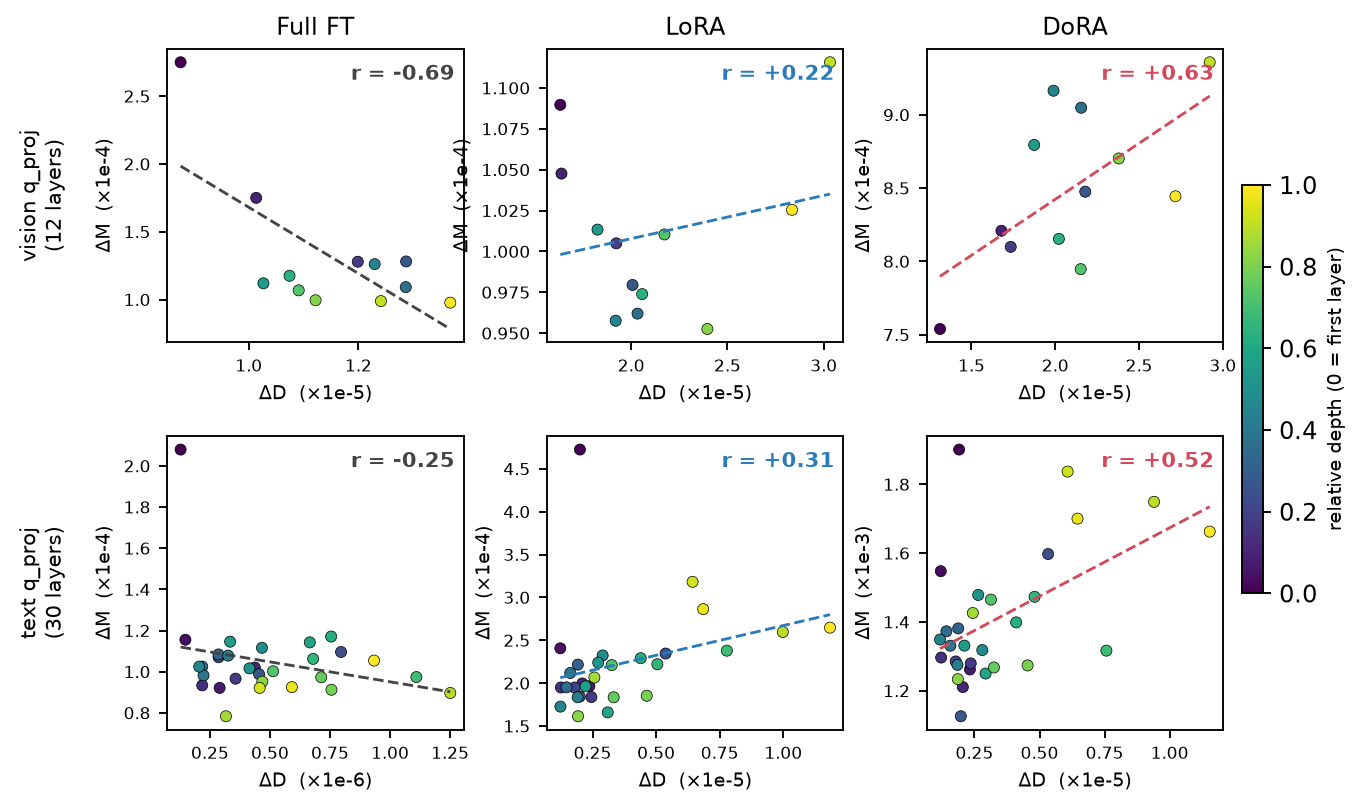
\includegraphics[width=0.8\linewidth]{fig_p1_final_ckpt.png}
  \caption{$\dM$ against $\dD$ for the query projection of each layer at the final checkpoint (step 250); colour shows layer depth.
    Full FT has the negative slope the paper reports.
    DoRA has the same positive slope as LoRA, in both the vision encoder (top) and the language model (bottom).}
  \label{fig:corr}
\end{figure}

\textbf{Interpretation.}
\begin{itemize}
  \item \textbf{The FT and LoRA half of the claim transfers} for the query projection, the matrix the paper analyses.
        FT is negative in both towers, most clearly in the vision encoder ($\rho=-0.50$; $r=-0.41$ with layer 0 removed), and LoRA is positive.
  \item \textbf{The DoRA half does not.} In every q and k projection DoRA's sign is positive. In both towers its per-layer pattern follows LoRA, not FT (Fig.~\ref{fig:corr}).
        Its answers do too: DoRA gives the same answer as LoRA on 265 of 300 questions, but the same as full FT on only 147.
  \item \textbf{DoRA decouples the two components only in scale.} For the same $\dD$ as LoRA in the vision encoder ($3.1\times10^{-5}$ for both), DoRA moves magnitude $8\times$ more ($8.8\times10^{-4}$ vs.\ $1.0\times10^{-4}$).
        The learned magnitude vector absorbs a uniform per-layer rescale, but it does not produce FT's trade-off between layers.
  \item \textbf{Outside q and k the signs are mixed} for every method, including FT's positive v and o projections, so the negative slope looks specific to the query and key projections.
  \item \textbf{Verdict: the hypothesis is partly refuted.} In SmolVLM, DoRA reproduces neither FT's $\dM$--$\dD$ pattern nor a reliable accuracy gain over LoRA.
\end{itemize}

\section{Bonus: the vision encoder adapts by rotating, not rescaling}
Under full FT, the relative direction change in the vision encoder is \textbf{32$\times$ larger} than in the language model ($\dD$ $1.4\times10^{-5}$ vs.\ $4.4\times10^{-7}$), while the magnitude change is about the same ($1.1\times10^{-4}$ vs.\ $0.9\times10^{-4}$).
With the low-rank methods the gap is $8\times$, and the negative FT slope is also clearest in the vision encoder.
One reading: SigLIP was pretrained on natural images, and document pages at 1024\,px are far from that distribution, so adapting the encoder means \emph{re-orienting} its query and key features toward small glyphs and layout rather than rescaling them.
This is the regime where DoRA's separate direction update should matter most, and the one the paper never examined.

\textbf{Tower ablation (causal test).}
DoRA was retrained with the same settings on one tower only, with the connector frozen (Table~\ref{tab:abl}).
\begin{table}[!htbp]
  \centering\small
  \begin{tabular}{lccccc}
    \toprule
    DoRA targets & Trainable & ANLS & $\Delta$ vs all-tower DoRA [95\% CI] & Vision $\dD$ & Text $\dD$ \\
    \midrule
    Both towers + connector & 1.7M & 57.5 & --  & $3.1\times10^{-5}$ & $3.9\times10^{-6}$ \\
    Vision encoder only     & 0.6M & \pending & \pending & \pending & -- \\
    Language model only     & 1.0M & \pending & \pending & -- & \pending \\
    \bottomrule
  \end{tabular}
  \caption{DoRA applied to a single tower.}
  \label{tab:abl}
\end{table}

\pending: interpretation of the ablation.

\section{Limitations}
\begin{itemize}
  \item One seed and one short run (250 steps); the paper trains far longer, and DoRA's negative slope may need more steps to appear.
  \item $\dD$ grows with the square of the update size and $\dM$ linearly, so matrices sit at different scales; correlations are therefore reported per projection.
  \item FT uses a 10$\times$ smaller learning rate than the adapters, a standard but uncontrolled choice.
  \item 12 vision layers give wide intervals on each $r$.
  \item \textbf{Code:} \code{part1\_vlm\_dora/} (\code{dora\_vlm.py}, \code{run\_colab.ipynb}) reproduces every number; figures come from \code{report/make\_p1\_figs.py}.
\end{itemize}

% ================================================================ PART 2
\clearpage
\section*{Part 2: LoRA fine-tuning a small LLM for tool calling}
\addcontentsline{toc}{section}{Part 2}
\small

\textbf{Setup.}
\begin{itemize}
  \item \textbf{Model:} Qwen2.5-0.5B-Instruct (494M parameters), using its native tool-calling chat template.
  \item \textbf{Tools} (made-up data): \code{calculator}, \code{convert\_units}, \code{get\_weather} (12 cities), \code{get\_stock\_price} (8 invented tickers), \code{days\_between}.
  \item \textbf{Agent loop:} generate a reply (greedy), parse \code{<tool\_call>\{json\}</tool\_call>}, run the tool and append the result as a \code{tool} message; stop on a plain-text reply or after 4 steps.
  \item \textbf{Data (templates):} 800 train requests (160 need no tool, 100 need a two-step chain: weather$\to$\textdegree F, price$\to$total) and 100 test requests (20 no tool, 20 two-step; 91 unique).
        Test phrasings come from separate templates, and test dates are written in words (``March 1, 2024'') while train uses ISO dates.
  \item \textbf{LoRA:} $r=16$, $\alpha=32$, dropout 0.05 on all linear layers (8.8M trainable, 1.8\%); lr $2\times10^{-4}$ cosine, batch 8, 2 epochs (200 steps), fp16 autocast; loss only on assistant turns (tool calls and final answers).
        Colab T4, seed 42, 8.1 min; train loss $0.60\to0.011$.
\end{itemize}

\textbf{Baseline vs.\ LoRA} (same 100 test requests, same system prompt):
\begin{center}
  \begin{tabular}{lccc}
    \toprule
    Metric & Base & Base + stronger prompt$^1$ & \textbf{LoRA} \\
    \midrule
    Call validity (parses in the expected format)       & 86.2 & 93.8 & \textbf{96.2} \\
    Call accuracy (right tool and arguments, in order)  & 52.5 & 56.2 & \textbf{93.8} \\
    Abstention (no call when none is needed, $n=20$)    & 60.0 & 25.0 & \textbf{100.0} \\
    Task success (final answer correct, end to end)     & 54.0 & 49.0 & \textbf{93.0} \\
    \quad two-step tasks only ($n=20$)                  & 10.0 & 0.0  & \textbf{100.0} \\
    \bottomrule
  \end{tabular}
\end{center}
{\footnotesize $^1$The stronger prompt adds a format example, ``never guess live values'', ``one tool at a time'' and ``dates as YYYY-MM-DD''.
This column was scored before a small scorer fix (keyword stemming; calls to non-existent tools counted as wrong tool, not wrong format), which changed base task success by only 2 points.\par}

\textbf{Failure analysis.}
Each failed request was assigned one category automatically and then checked by hand.
The base model fails 46 of 100 requests and LoRA fails 7; LoRA has fewer than 10 failures, so all 7 are listed.
\begin{center}
  \begin{tabularx}{\linewidth}{lccY}
    \toprule
    Category & Base & LoRA & Typical base behaviour \\
    \midrule
    Incomplete chain & 12 & 0 & Gets the weather in \textdegree C, then answers without converting to \textdegree F; gets the price but never multiplies by the number of shares. \\
    Missed call      & 11 & 3 & Asks the user for the data (``please tell me the ticker'') or makes up a price (``\$50 per share''). \\
    Unnecessary call &  8 & 0 & Calls \code{get\_weather("New York")} for ``Who first walked on the Moon?'' \\
    Wrong argument   &  7 & 0 & Wrong date range, unit direction reversed, \code{993 + 40 * 9} instead of \code{(993 + 40) * 9}, typo \code{NIBM}. \\
    Wrong tool       &  6 & 2 & \code{get\_weather(city="KRYO")} for a stock; invents \code{split\_into\_parts}. \\
    Wrong answer (no tool needed) & 2 & 2 & -- \\
    \bottomrule
  \end{tabularx}
\end{center}

\textbf{What LoRA fixed, kept and introduced.}
\begin{itemize}
  \item \textbf{Fixed (39 of 46):} every incomplete chain, unnecessary call and wrong argument, 8 of 11 missed calls and 4 of 6 wrong-tool cases.
        LoRA learned to chain a second call after reading the first result, to leave general-knowledge questions alone, and to copy argument values exactly.
  \item \textbf{Kept (7):} three test phrasings unlike anything in training.
        ``Split 180 into 45 equal parts'' (2): both models invent a \code{split\_into\_parts} tool.
        ``Before I invest, tell me what NIMB costs per share'' (3): LoRA says it has no real-time data, or makes up a price.
        ``Which country is home to Kyoto?'' (2, a duplicated request): LoRA answers ``Kyoto is home to the city of Kyoto''.
  \item \textbf{Introduced:} none; no request that the base model solved fails after fine-tuning.
\end{itemize}

\textbf{Could a better prompt alone have been enough? No.}
The stronger prompt raised format validity (86$\to$94\%) but made the base model call tools far too often (abstention 60$\to$25\%, unnecessary calls 8$\to$15), and it did not teach chaining (two-step success 10$\to$0\%, 18 incomplete chains).
At 0.5B parameters, instructions shift the overall tendency to call a tool but do not teach \emph{when} to call; showing the full call$\to$result$\to$answer pattern through LoRA does.
Caveat: test requests share the tool set, cities and tickers of training, so the 93\% measures how well this tool set was learned, not tool use in general.

\normalsize
\begin{thebibliography}{9}\small
  \bibitem{dora} S.-Y. Liu, C.-Y. Wang, H. Yin, P. Molchanov, Y.-C.~F. Wang, K.-T. Cheng, and M.-H. Chen.
    DoRA: Weight-decomposed low-rank adaptation. \emph{arXiv:2402.09353}, 2024.
\end{thebibliography}

\end{document}
